\documentclass{article}
\usepackage{pdfpages}
\usepackage[backend=bibtex, sorting=ynt,maxbibnames = 10,citestyle = ieee]{biblatex}


\bibliography{/home/sr/svn/forsyte-publications/trunk/rubin.bib}
\DefineBibliographyStrings{english}{%
references = {},
 }

\usepackage{enumitem}% http://ctan.org/pkg/enumitem
\usepackage{hyperref}

\title{MAGNIFICO RETTORE\\
UNIVERSITA' DI PISA\\
LUNGARNO PACINOTTI, 43\\
56126 PISA\\
Selection code RIC2017a1\\
}
\date{27 July 2017}

\def\lb{\vfill{The rest of this page is intentionally left blank}\vfill}

\newif\ifcopy
\copyfalse

\begin{document}

\maketitle
\tableofcontents

\newpage

% {\center \section{Resunto}}
{\center \section{Overview}}

%\addcontentsline{toc}{section}{Overview}

\def\apptitle{Domanda titoli e pubblicazioni :  procedura di selezione per contratto a tempo determinato}
\def\selectioncode{A11}

\textbf{\apptitle}

\vspace{1cm}

\begin{tabular}{ l  l }
Department \dotfill & Information Engineering \\
Competitive Sector \dotfill &   09/H1\\
S.S.D \dotfill &  ING-INF/05\\
Applicant Surname \dotfill & Rubin \\
Applicant First Name \dotfill & Sasha\\
Applicant Residence \dotfill &  via Corigliano, 8, 80136, Napoli\\
\end{tabular}


% Personal details:
% \begin{tabular}{ l  l }
%  Surname \dotfill & Rubin \\
%  Name \dotfill & Sasha\\
%  Date of birth \dotfill & 16/02/1976\\
%  Place of birth \dotfill &  Johannesburg, Sud Africa\\
%  Citezenship \dotfill &  Nuova Zelanda\\
%  Codice Fiscale \dotfill & RBNSSH76B16Z347C\\
% \end{tabular}

% 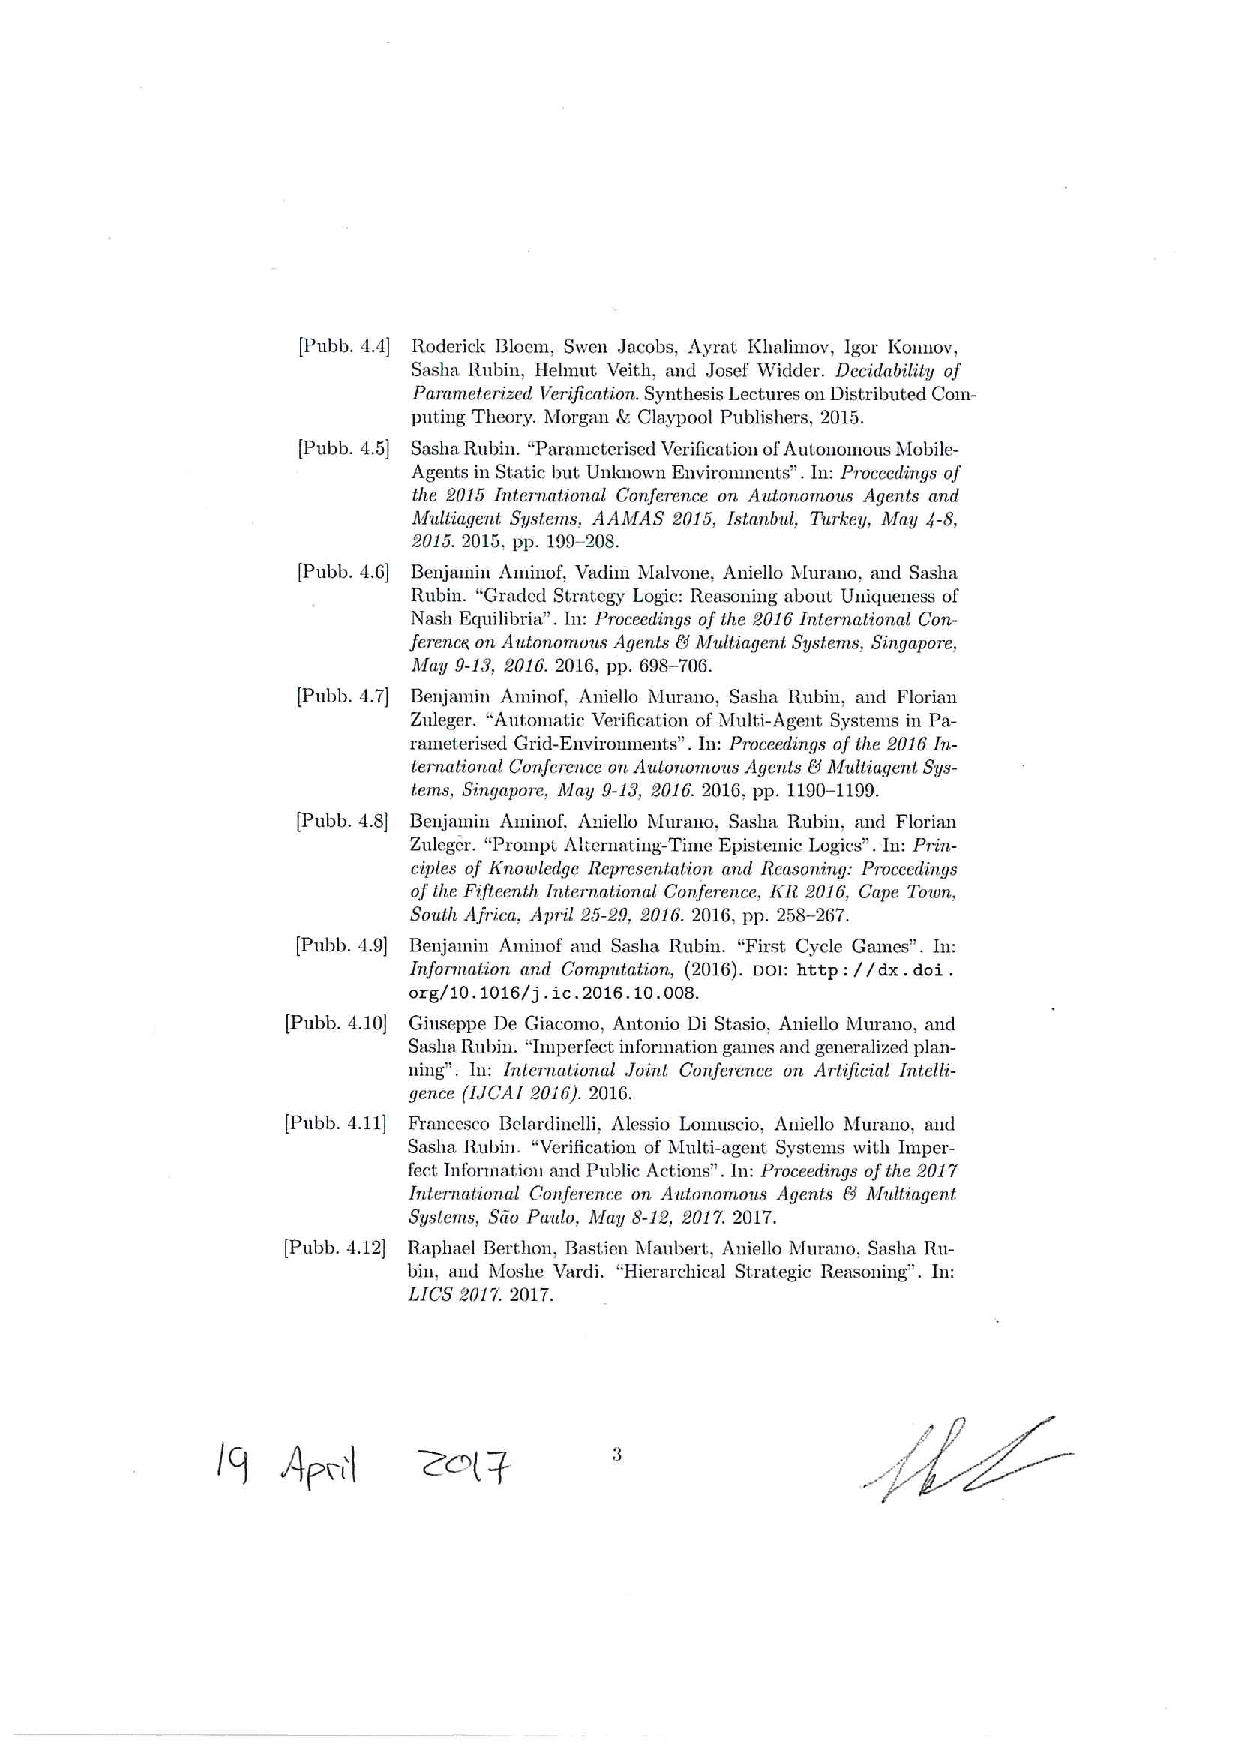
\includepdf[pages={-}, addtotoc={1, section, 1, List of enclosed documents}, }]{elenco.pdf}

{\center \section{List of enclosed documents}}


\begin{enumerate}
 \item[{[}3.1{]}] Autocertification
 \item[{[}3.2{]}] CV 
 \item[{[}3.3{]}] Passport ID
 \item[{[}3.4{]}] Codice Fiscale
\end{enumerate}

% [{[}Tesi $1${]}] 

\nocite{BMMRV17, BLMR17, GMRS16IJCAI}
%  DBLP:conf/kr/AminofMRZ16, DBLP:conf/atal/AminofMRZ16, DBLP:conf/atal/AminofMMR16, AR16, DBLP:series/synthesis/2015Bloem, DBLP:conf/prima/RubinZMA15, DBLP:conf/atal/Rubin15, BGR11, DBLP:journals/bsl/Rubin08}


{\small \printbibliography[prefixnumbers={Pubb. 4.}]
}
 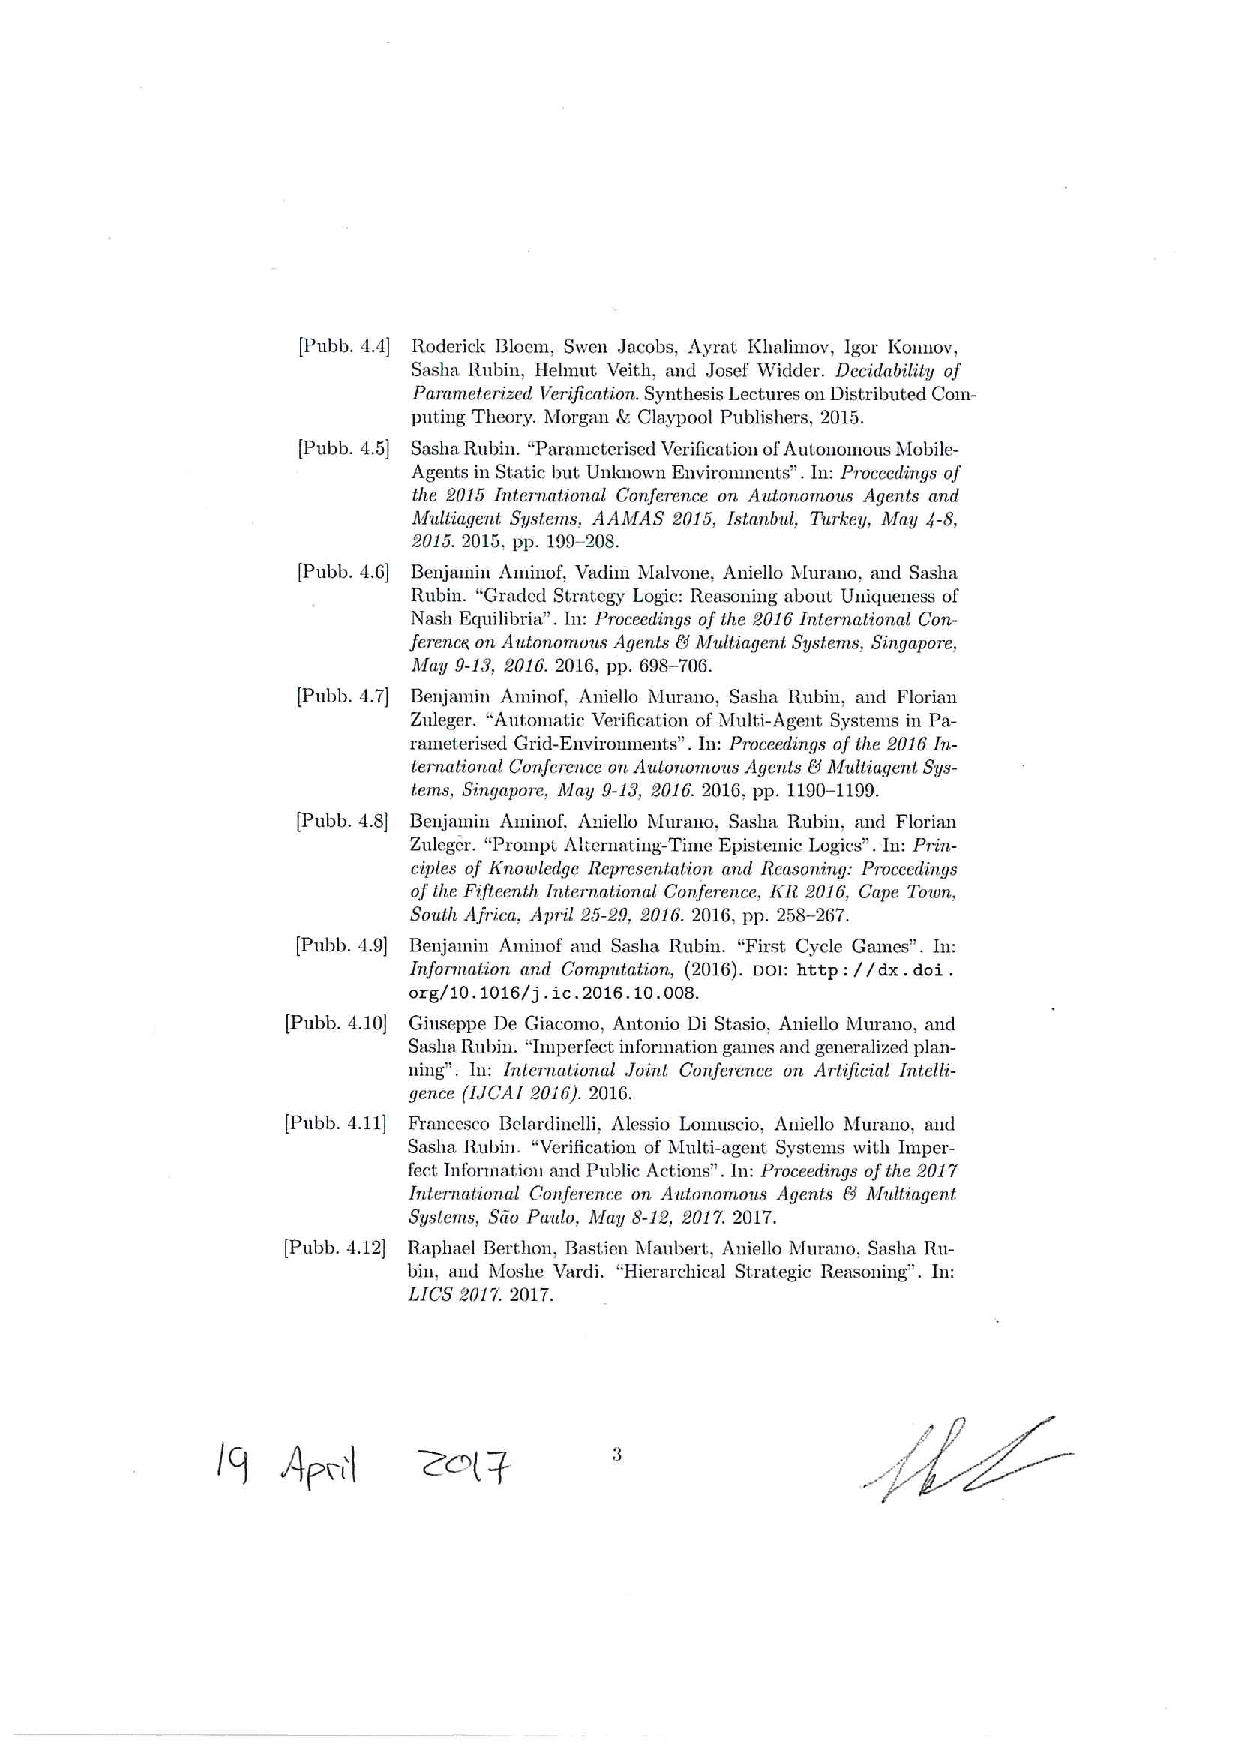
\includepdf[pages={-}]{elenco.pdf}


\newpage

\section{Attachments}

 \includepdf[pages={-}, addtotoc={1, subsection, 1, Autocertification), }]{autocertification.pdf}

\newpage

  \includepdf[pages={-}, addtotoc={1, subsection, 1, CV, }]{CV-Italian.pdf}
  \newpage
  
 % Instead of allegatoD write: allego autocertificazione per ogni documento dell'elenco
 

\includepdf[pages={-}, addtotoc={1, subsection, 1, Passport, }]{/home/sr/JOBS/aa-documents/PP-signed-dated.pdf}
% \section{ID} [To be included, a signed and dated copy of the front page of my passport] \newpage

\includepdf[pages={-}, addtotoc={1, subsection, 1, Codice Fiscale, }]{/home/sr/JOBS/aa-documents/CF.pdf}


\includepdf[pages={-}, addtotoc={1, subsection, 1, PhD Certificate, }]{/home/sr/JOBS/aa-documents/phd-certificate.jpg}


% \lb
% 
% 
\includepdf[pages={-}]{Thesis-Rubin.pdf}

% [prefixnumbers={Pubb.}]


\center \section{Publications}
\lb

\newpage
\center \subsection{Publications} 
 \lb 
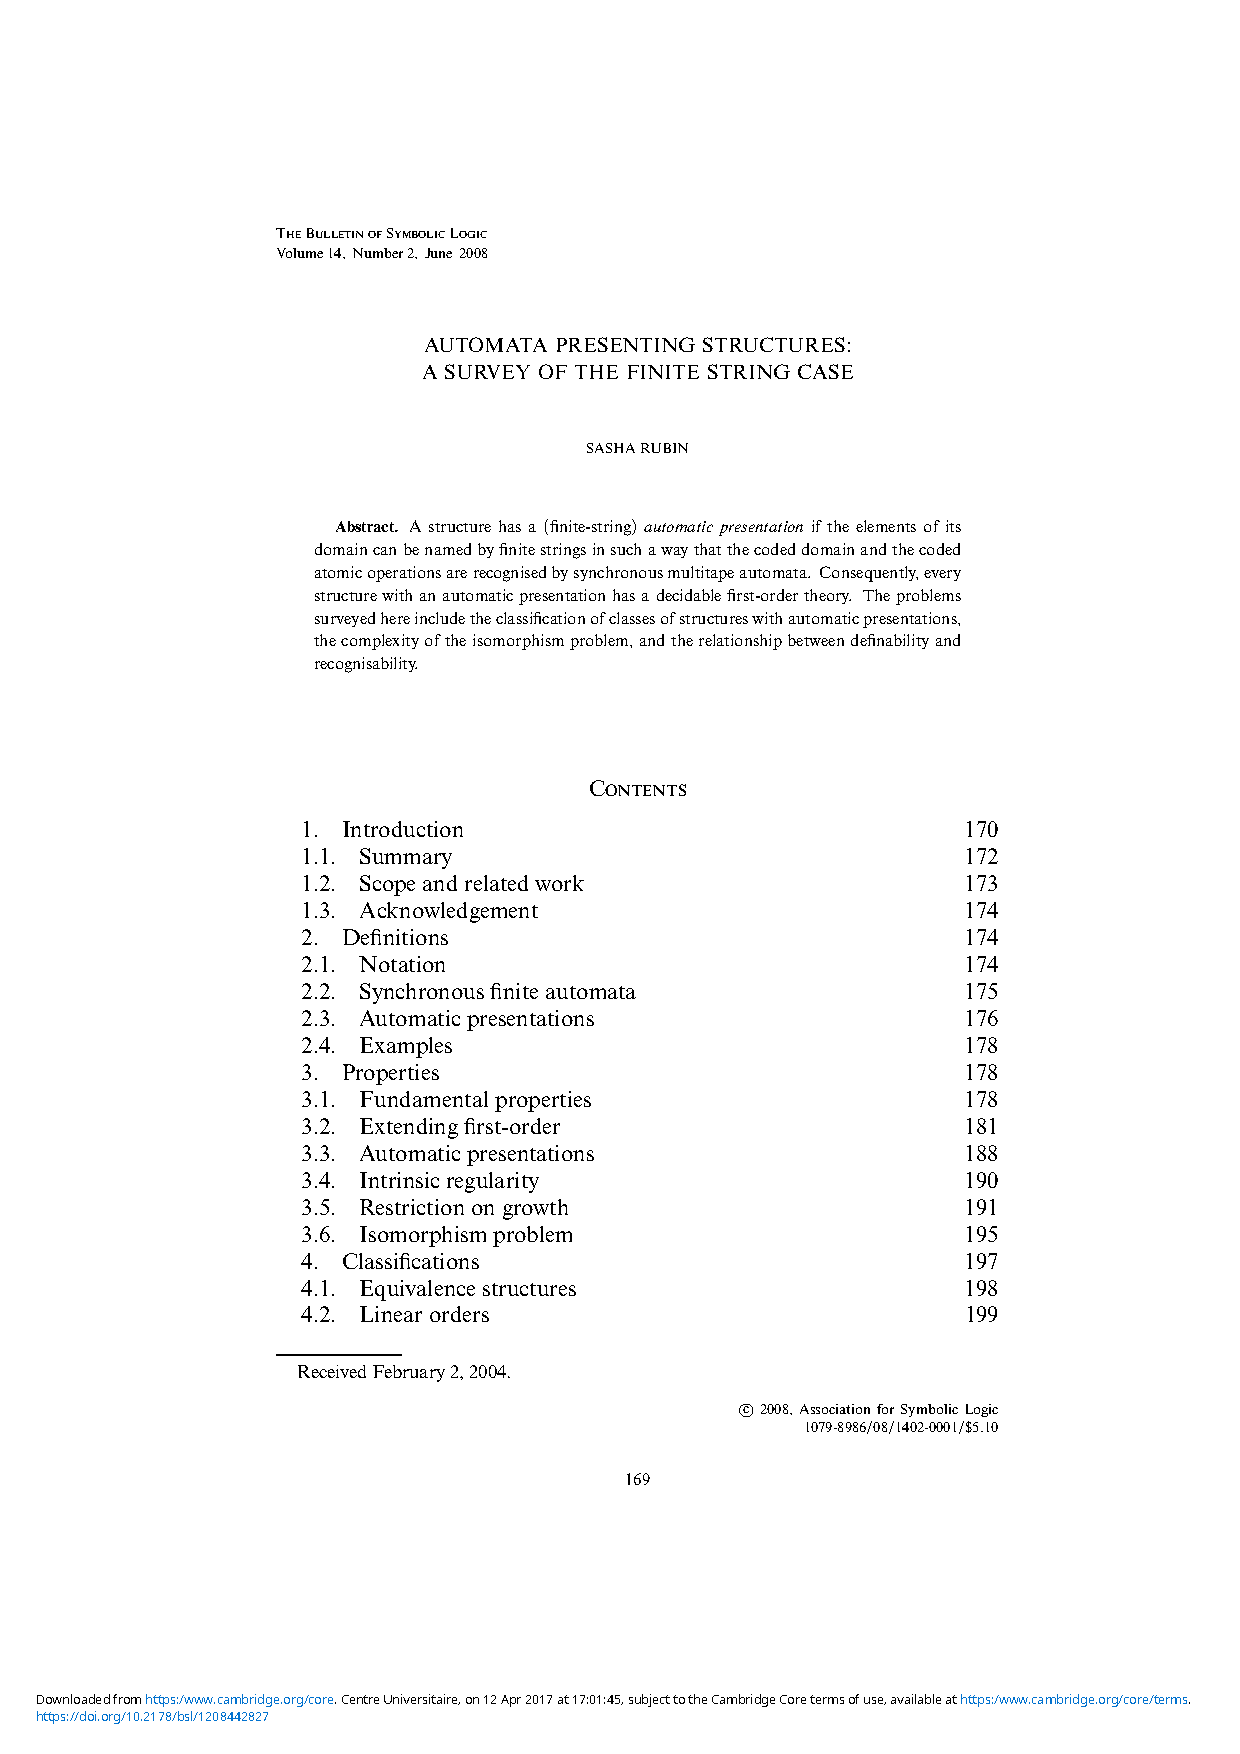
\includepdf[pages={-}]{no11.pdf}
\center \subsection{Publication} 
 \lb 
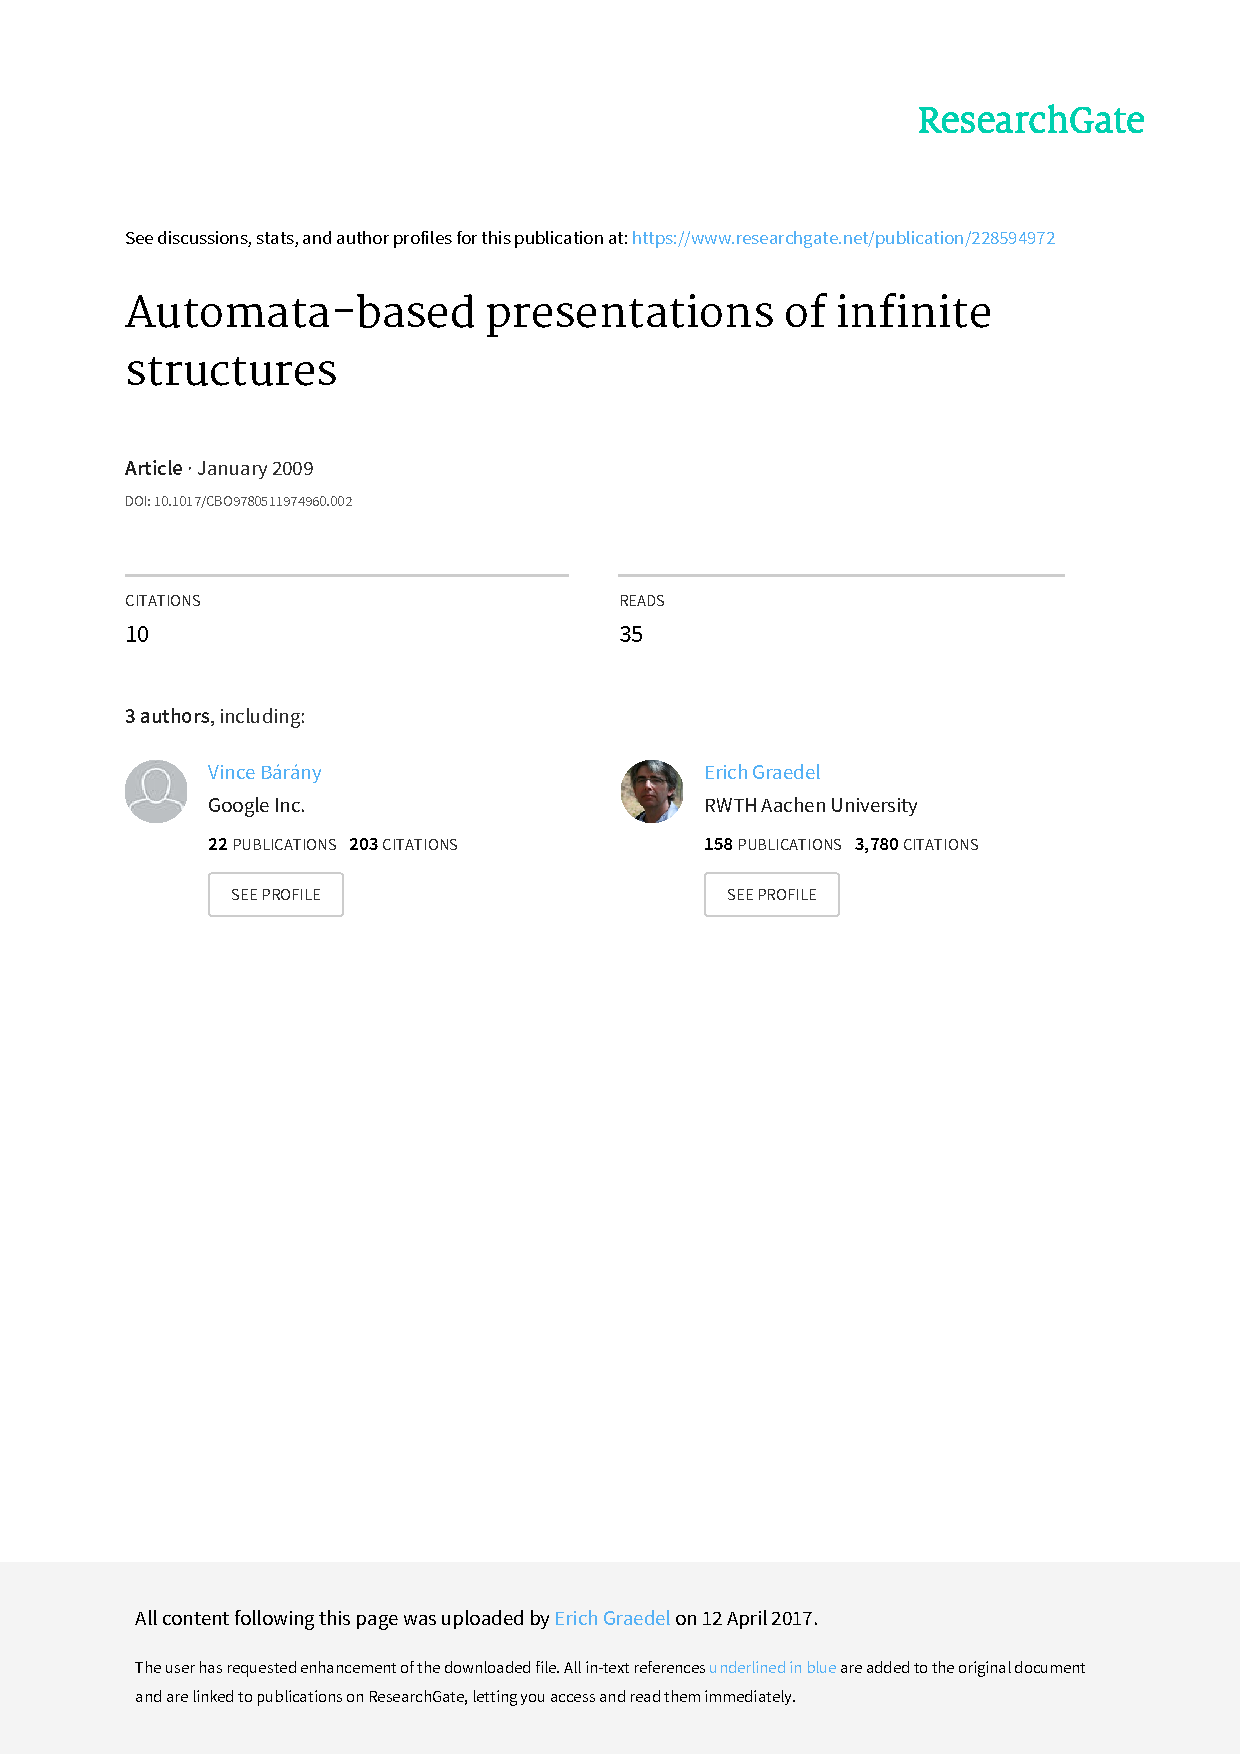
\includepdf[pages={-}]{no12.pdf}
\center \subsection{Publication} 
 \lb 
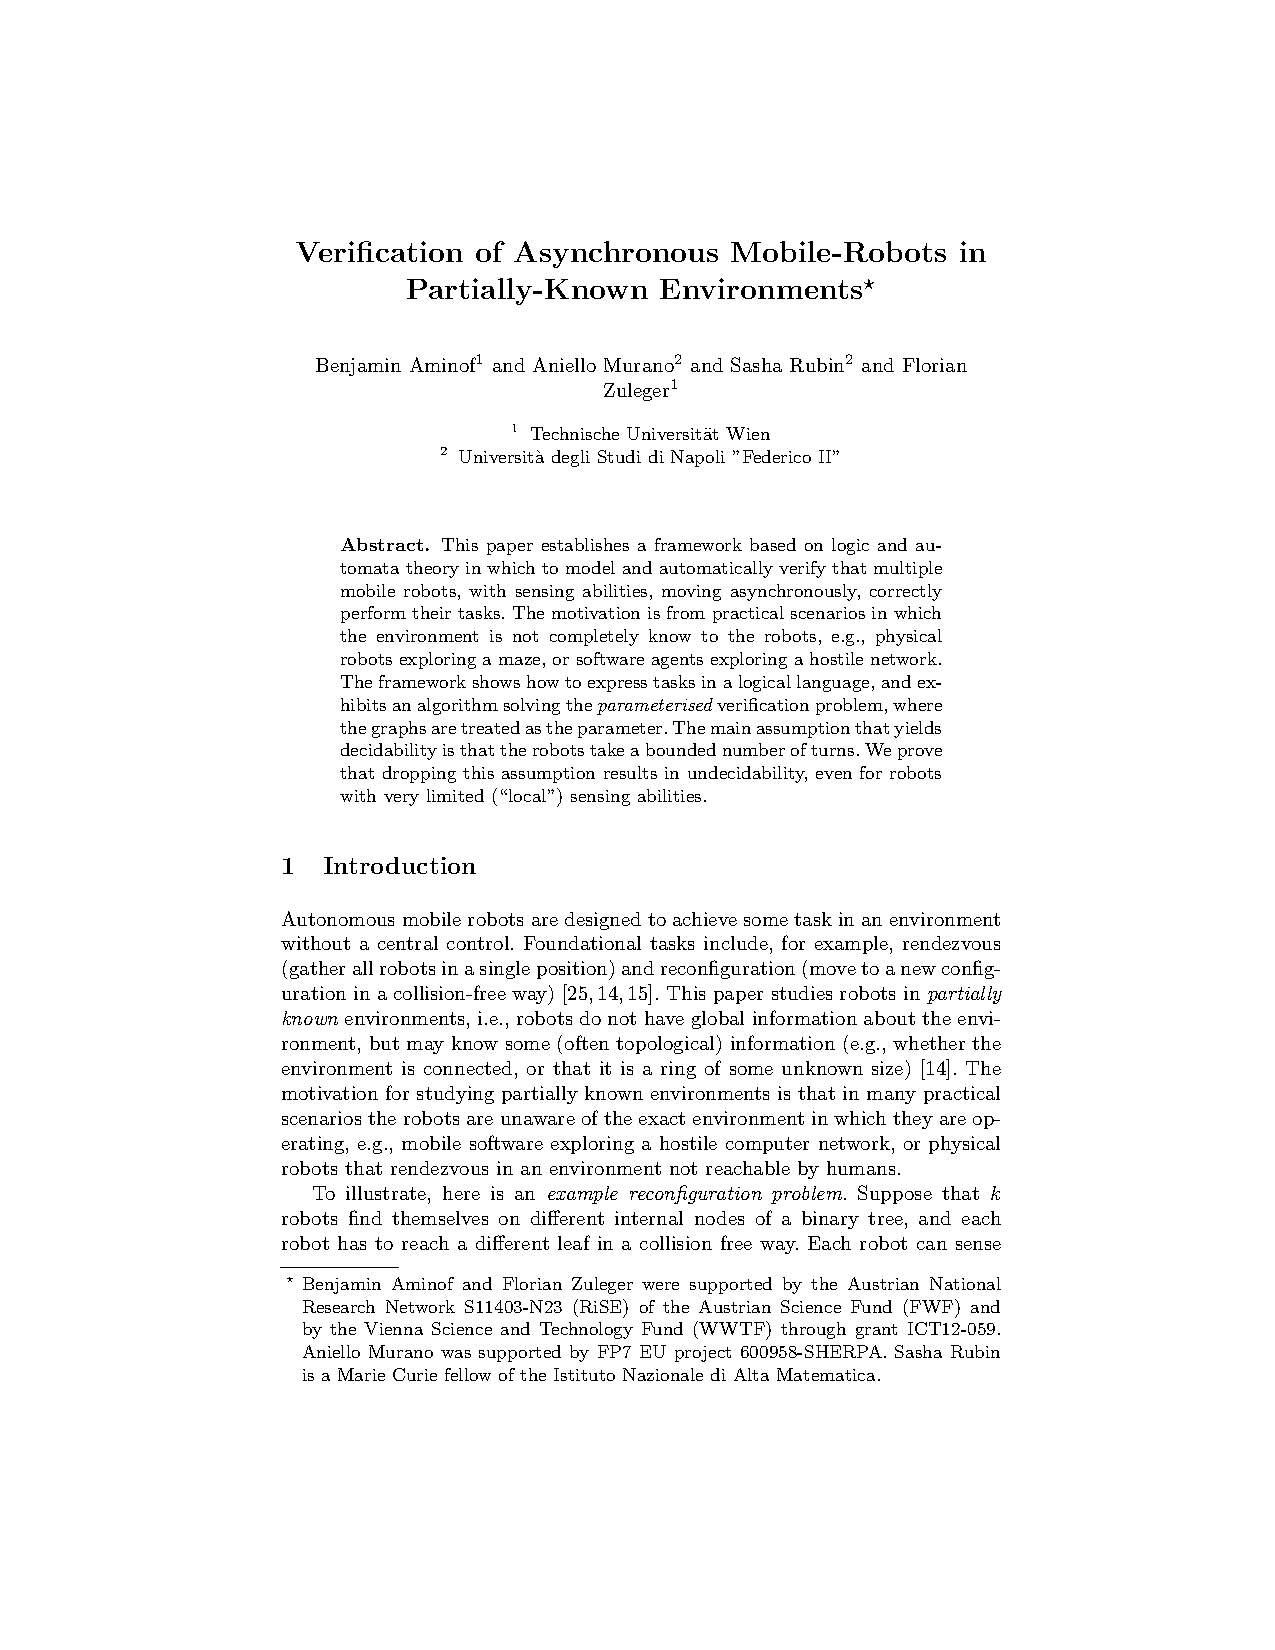
\includepdf[pages={-}]{no21.pdf}
\center \subsection{Publication} 
 \lb 

\includepdf[pages={-}]{no24.pdf}
\center \subsection{Publication} 
 \lb 
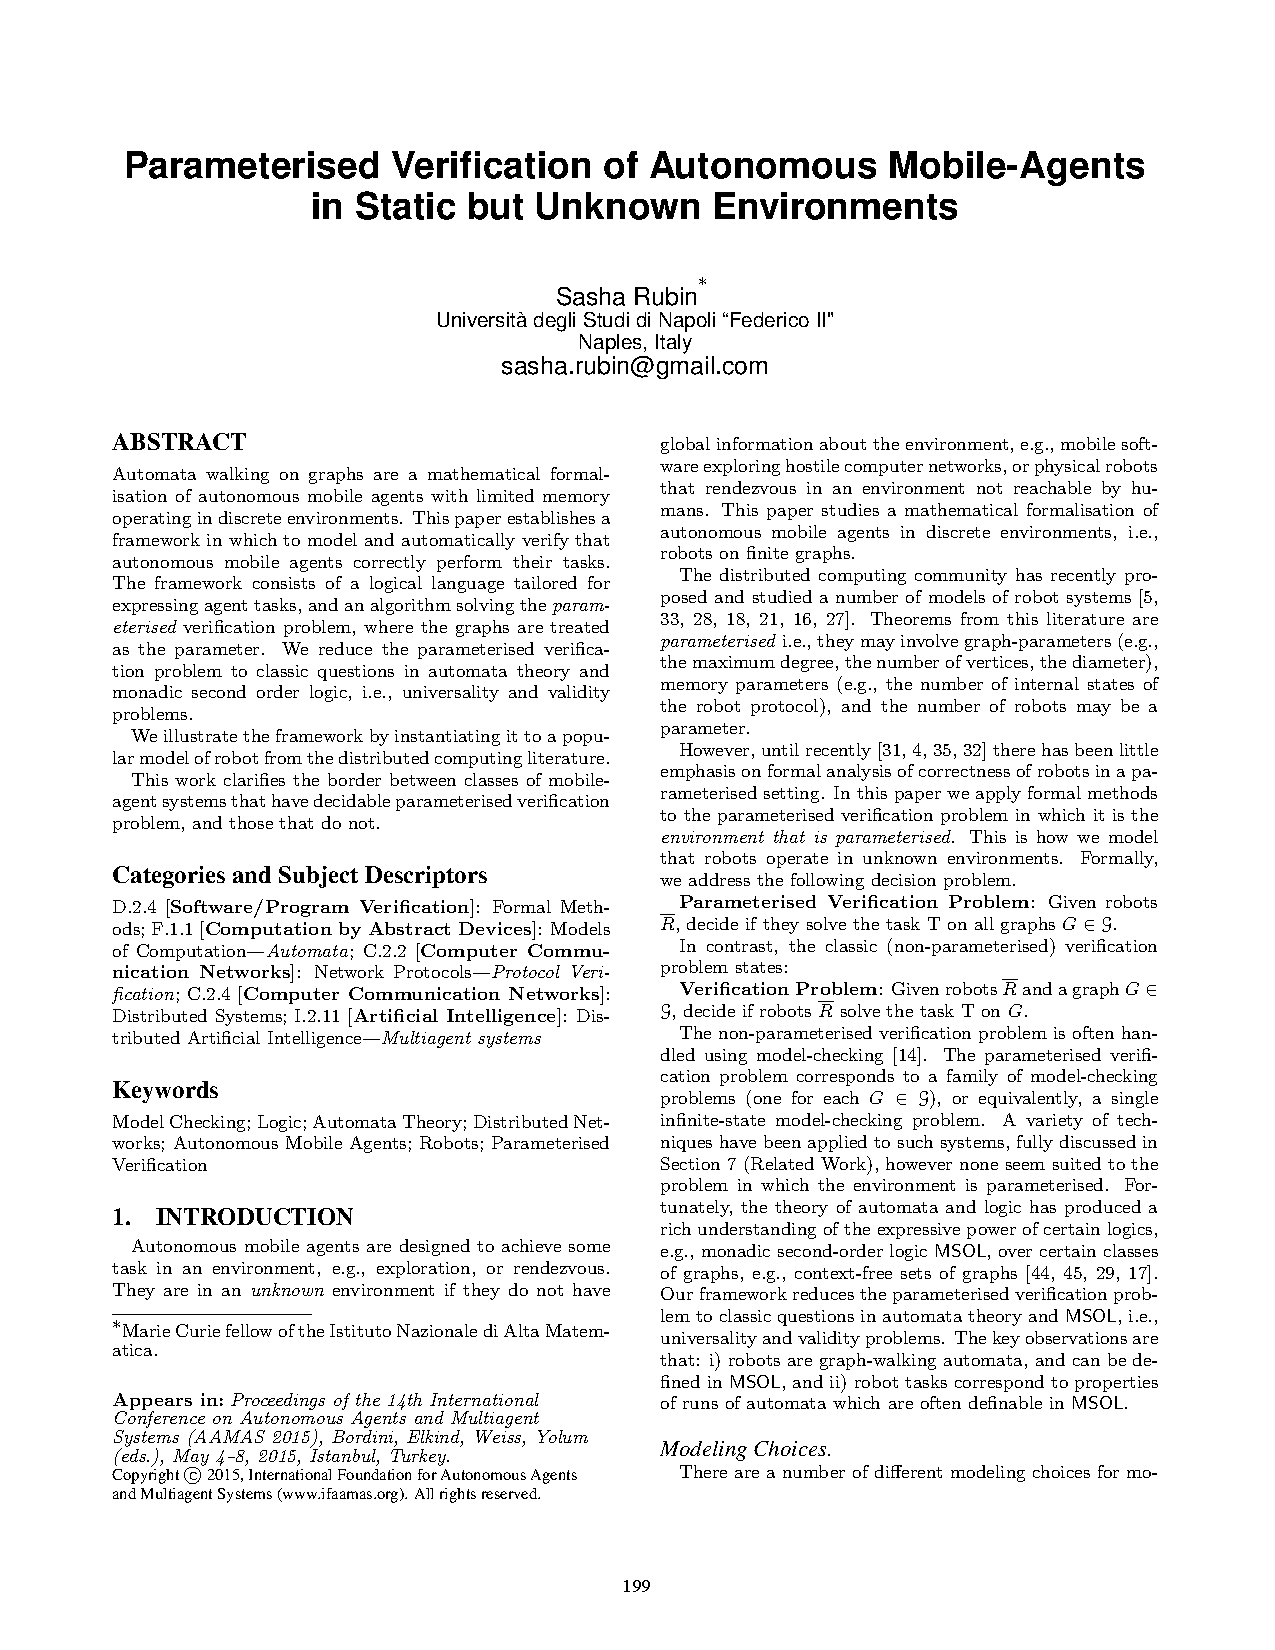
\includepdf[pages={-}]{no26.pdf}
\center \subsection{Publication} 
 \lb 
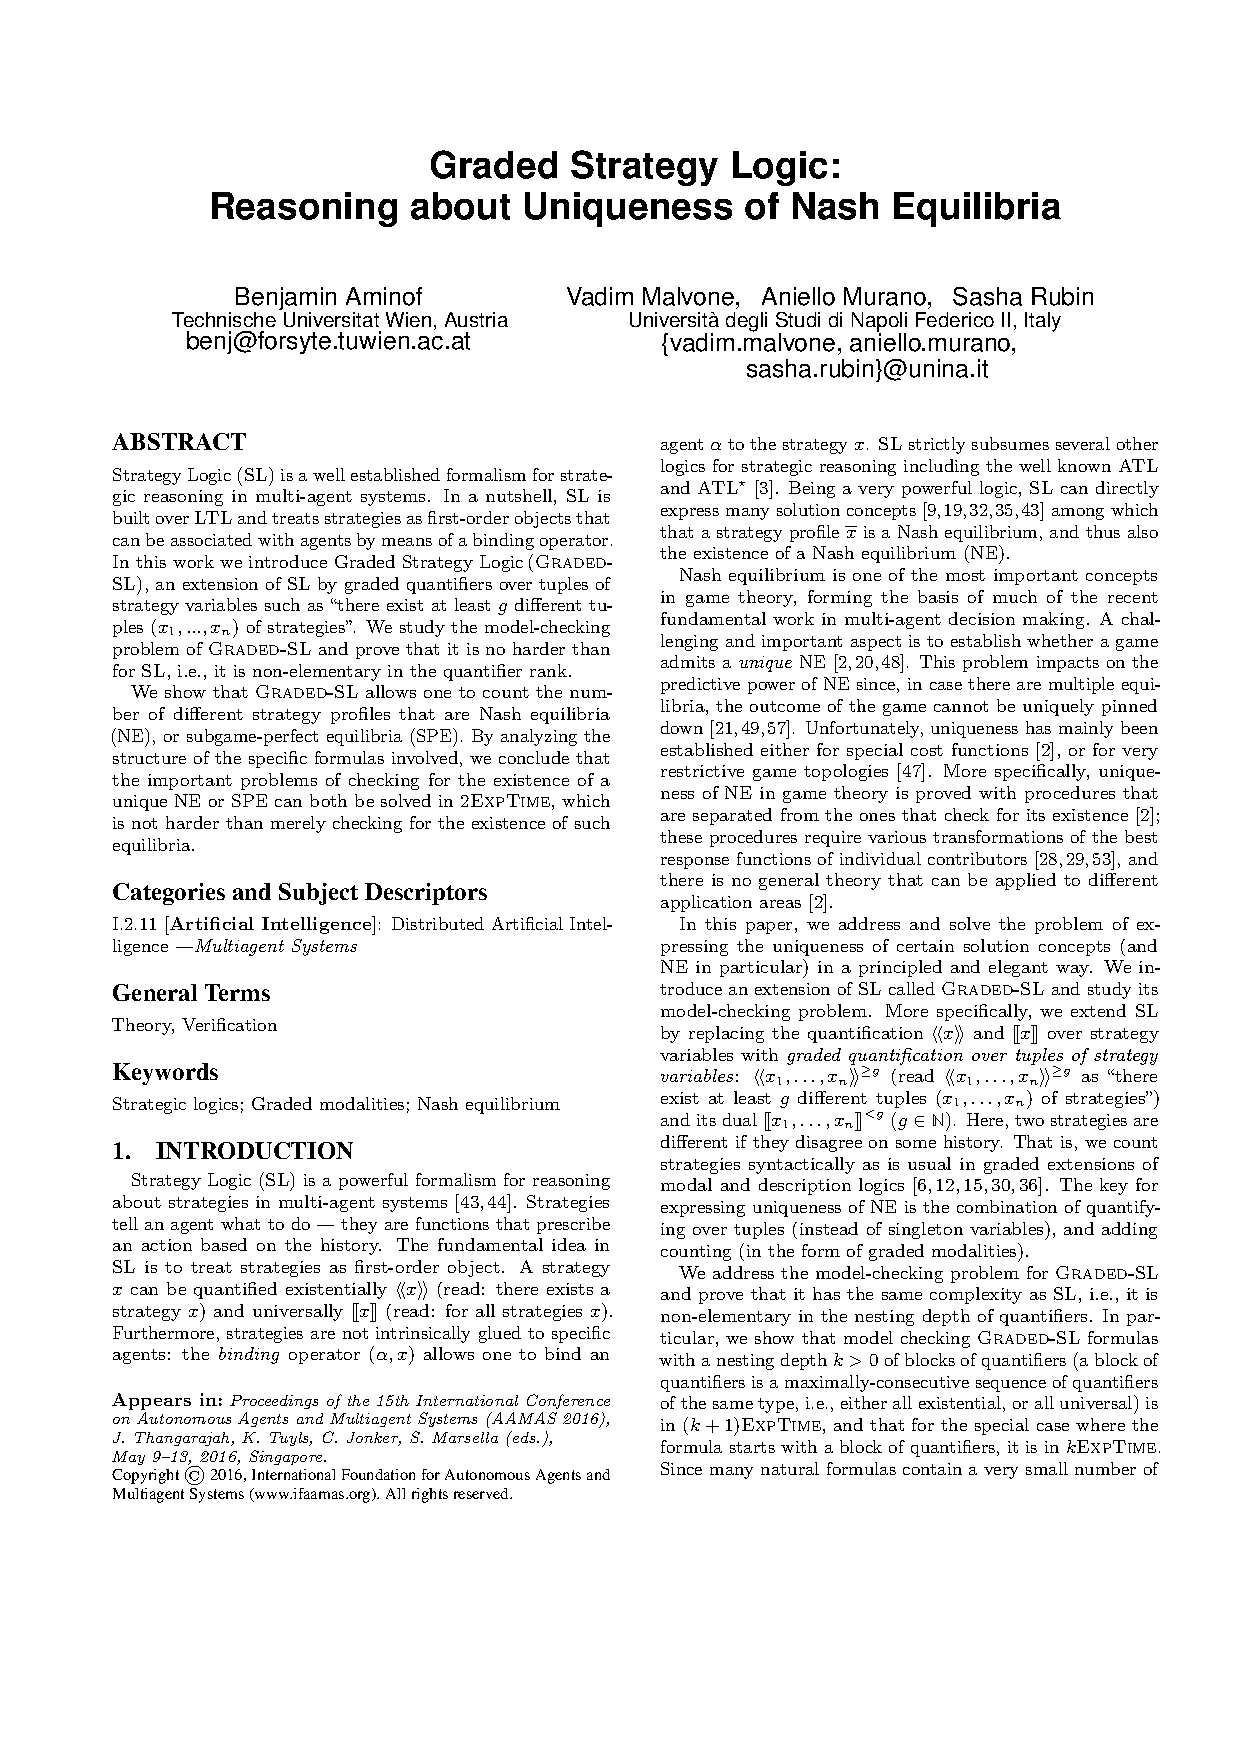
\includepdf[pages={-}]{no28.pdf}
\center \subsection{Publication} 
 \lb 
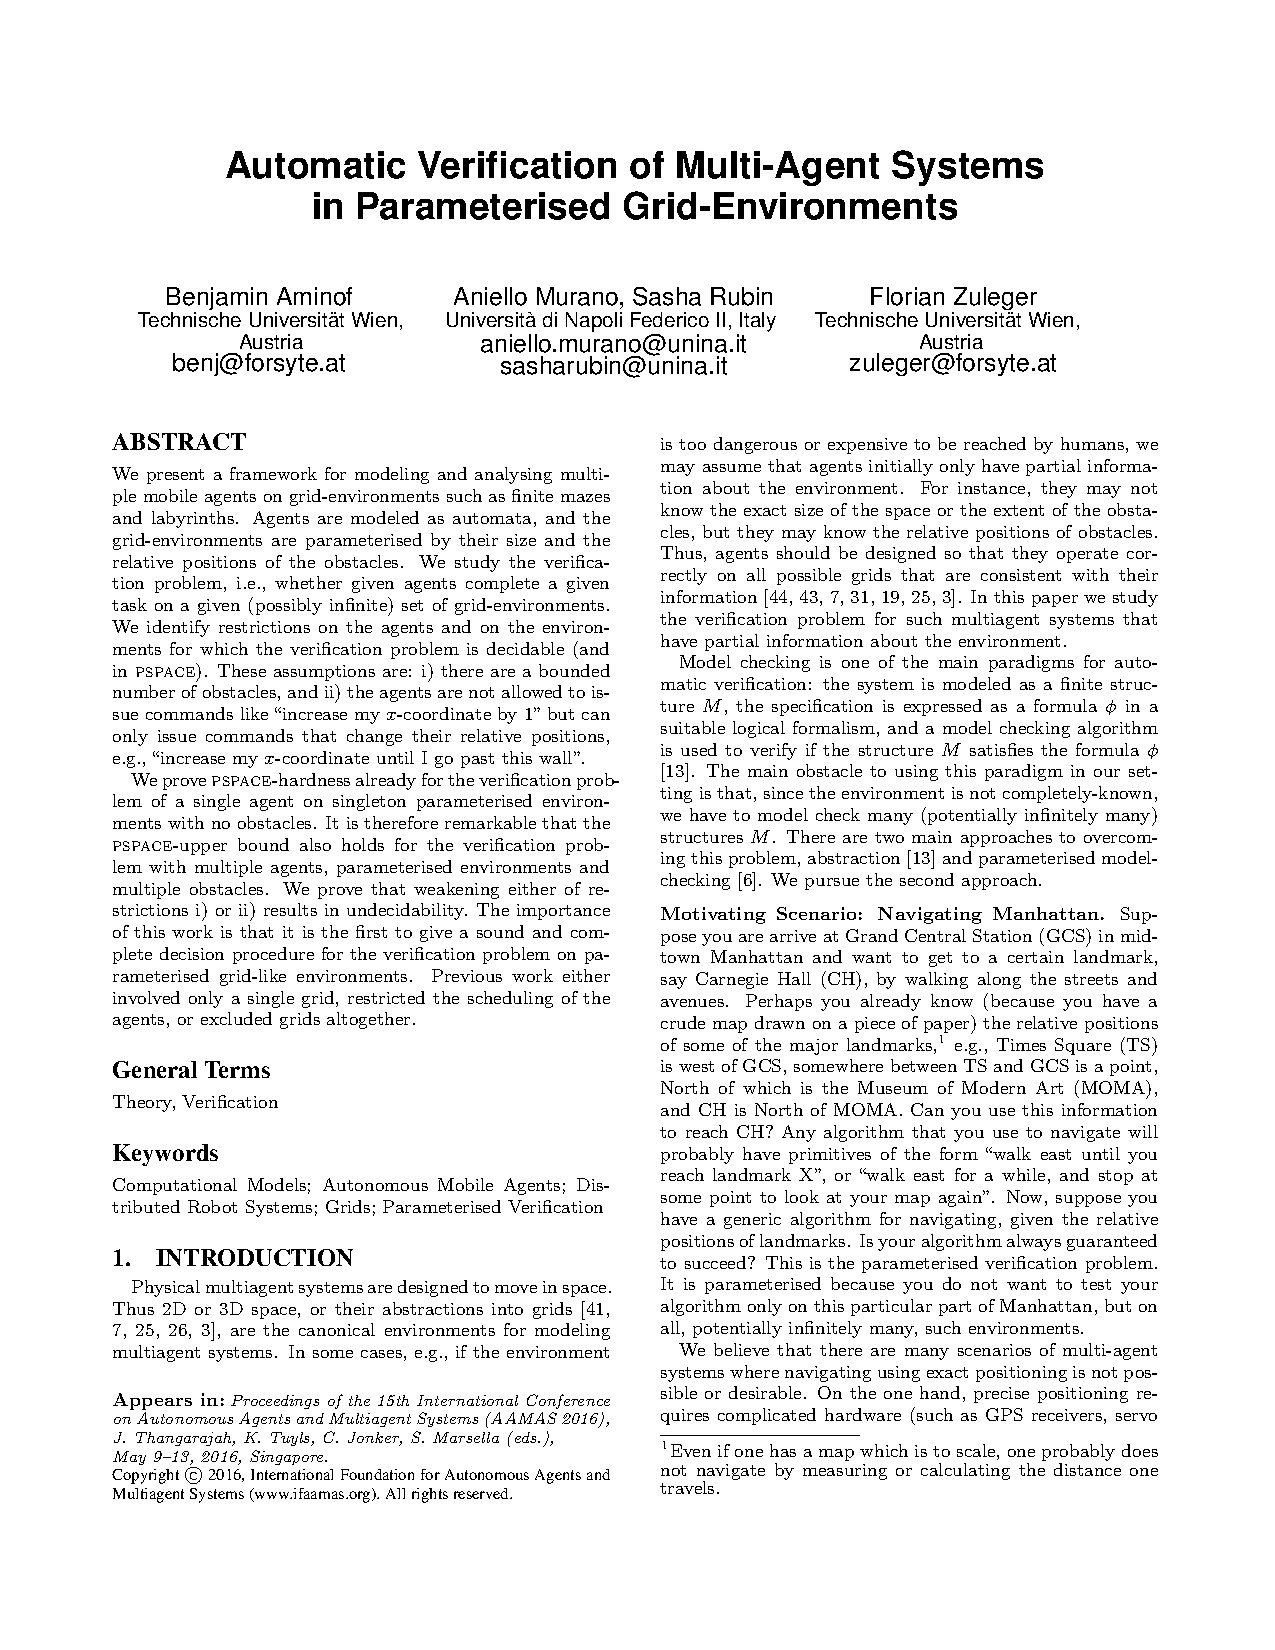
\includepdf[pages={-}]{no29.pdf}
\center \subsection{Publication} 
 \lb 
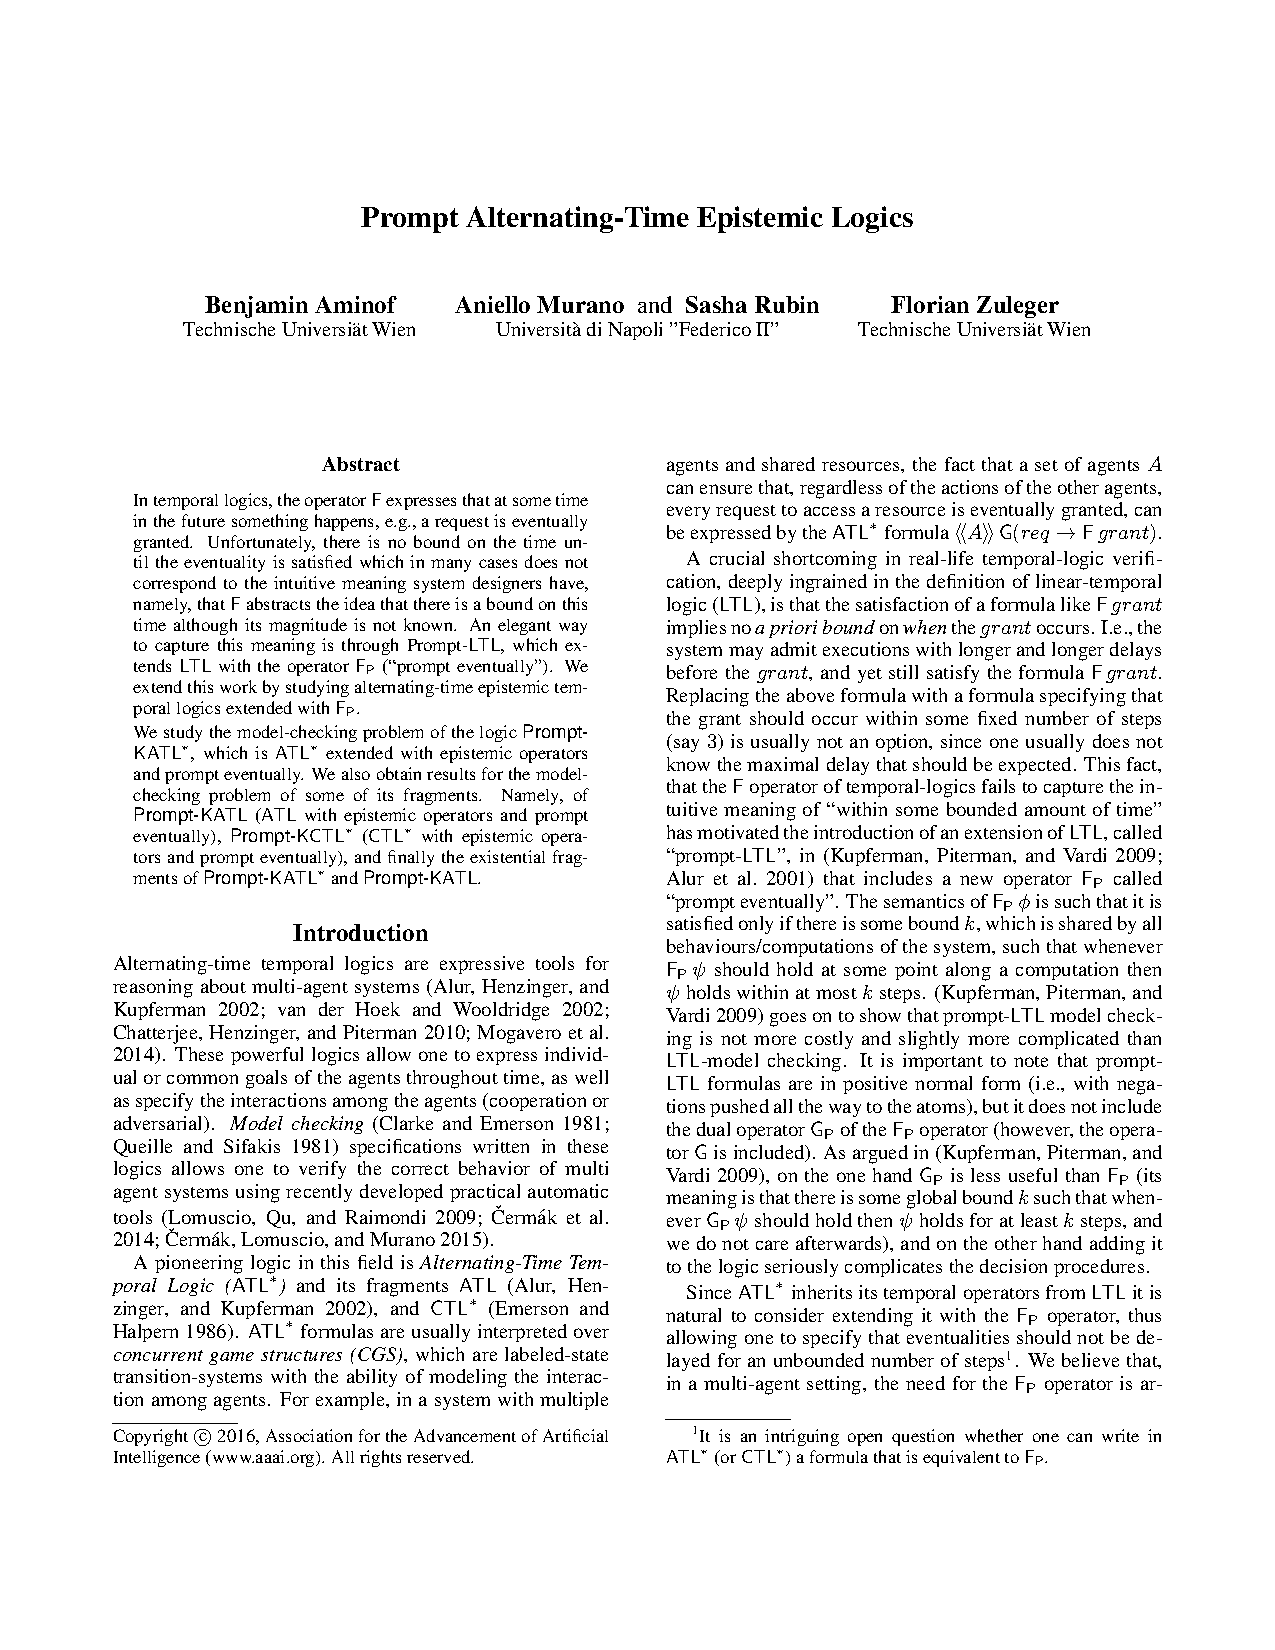
\includepdf[pages={-}]{no30.pdf}
\center \subsection{Publication} 
 \lb 
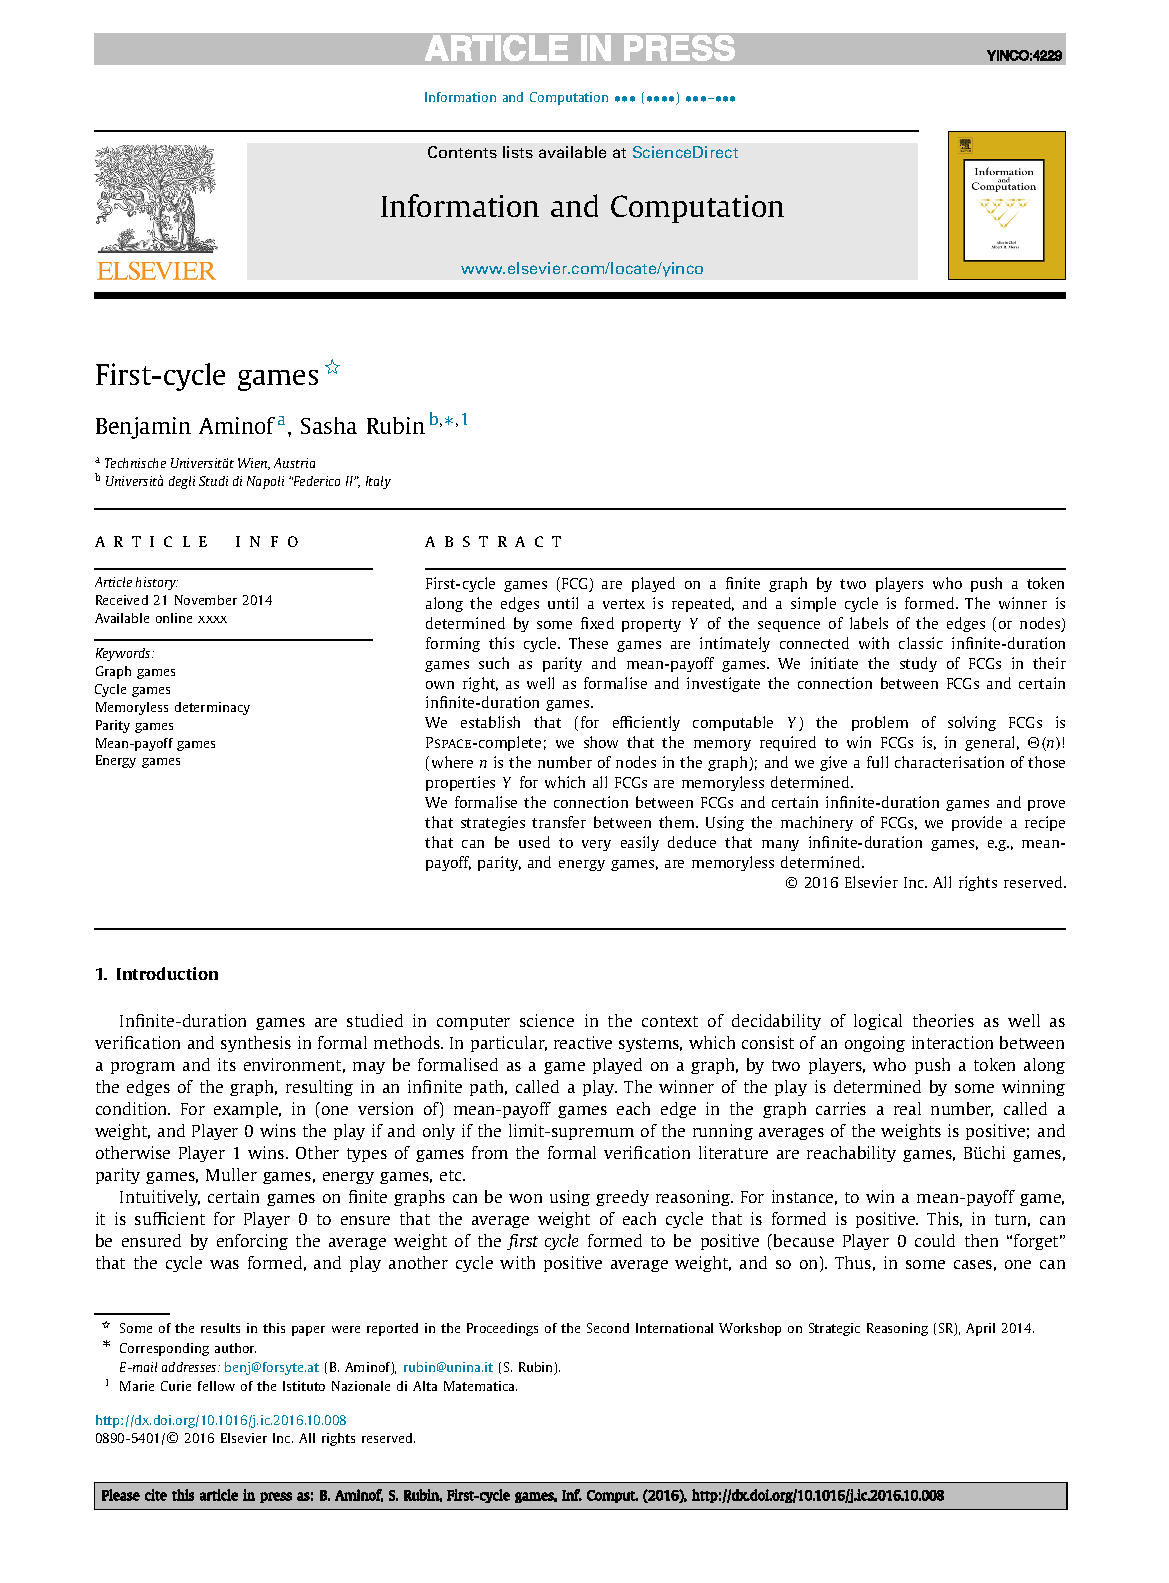
\includepdf[pages={-}]{no31.pdf}
\center \subsection{Publication} 
 \lb 
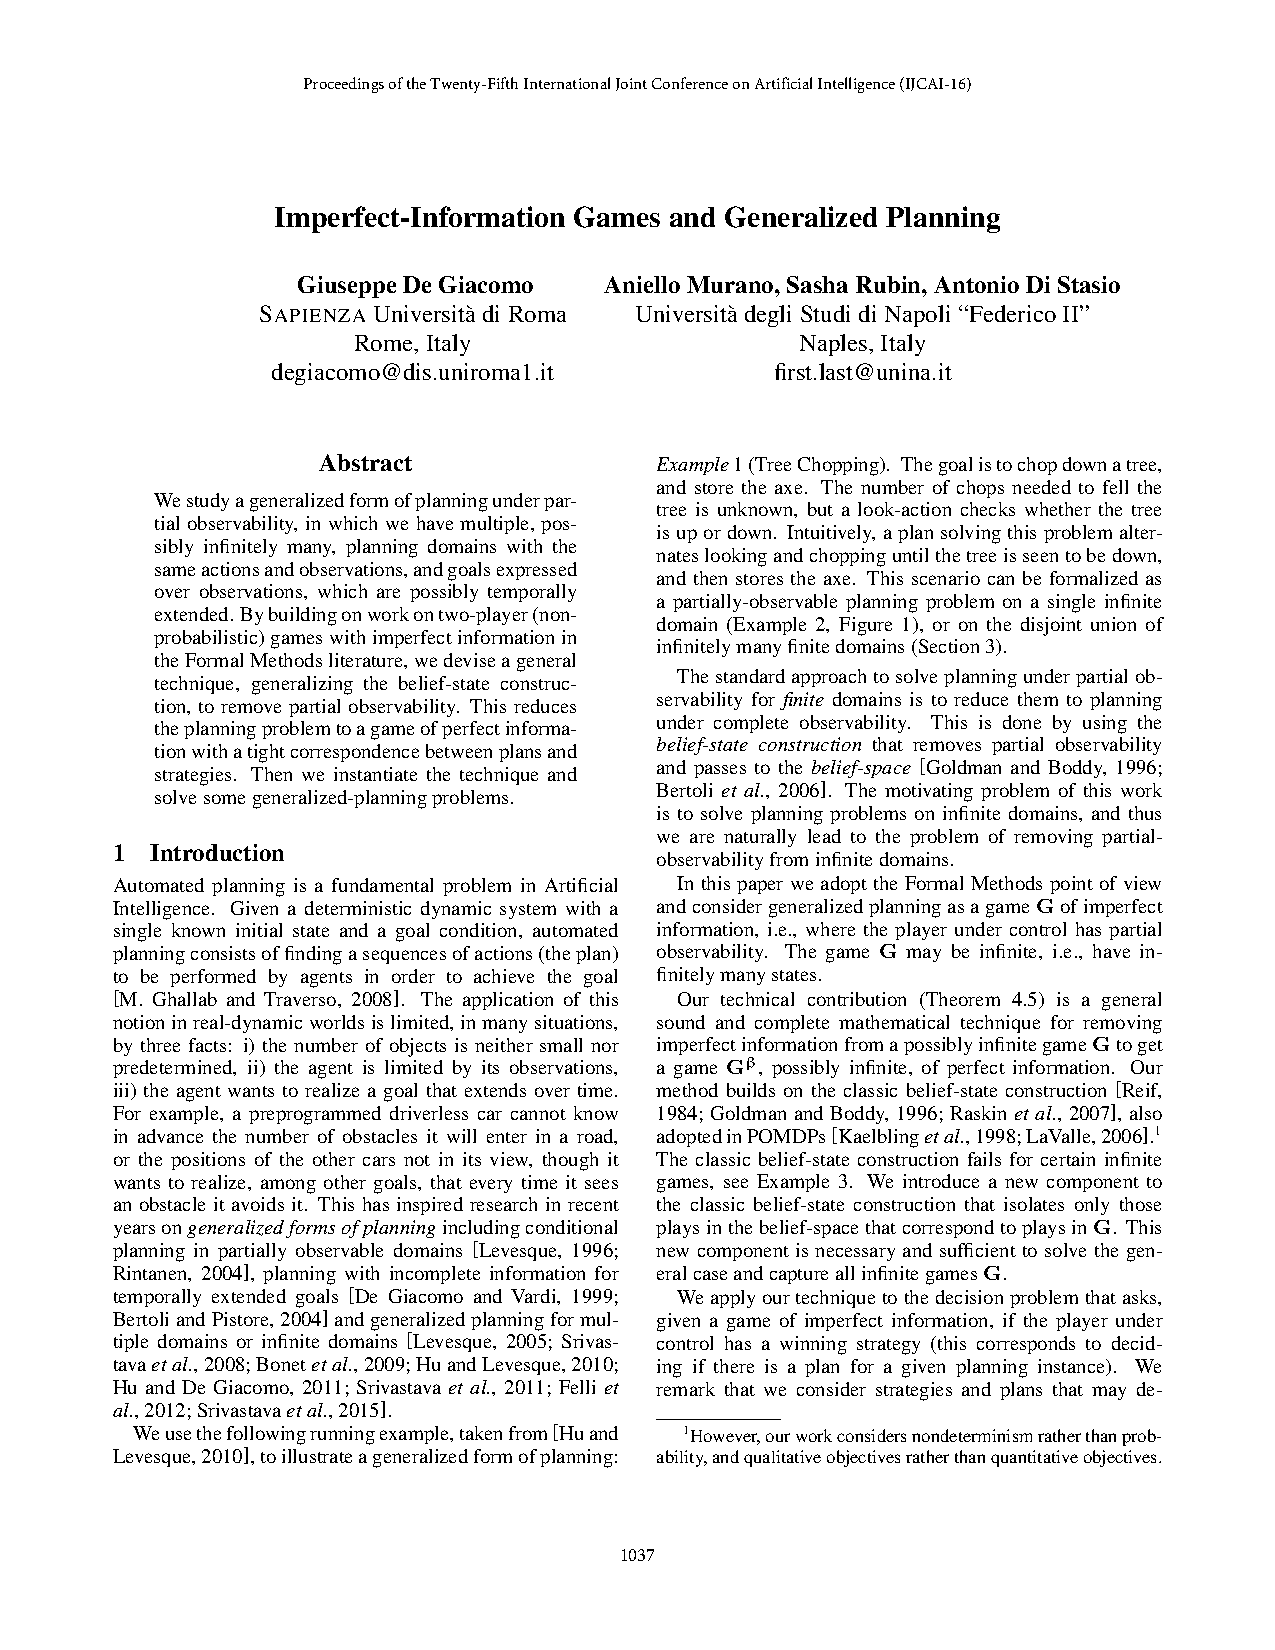
\includepdf[pages={-}]{no34.pdf}
\center \subsection{Publication} 
 \lb 
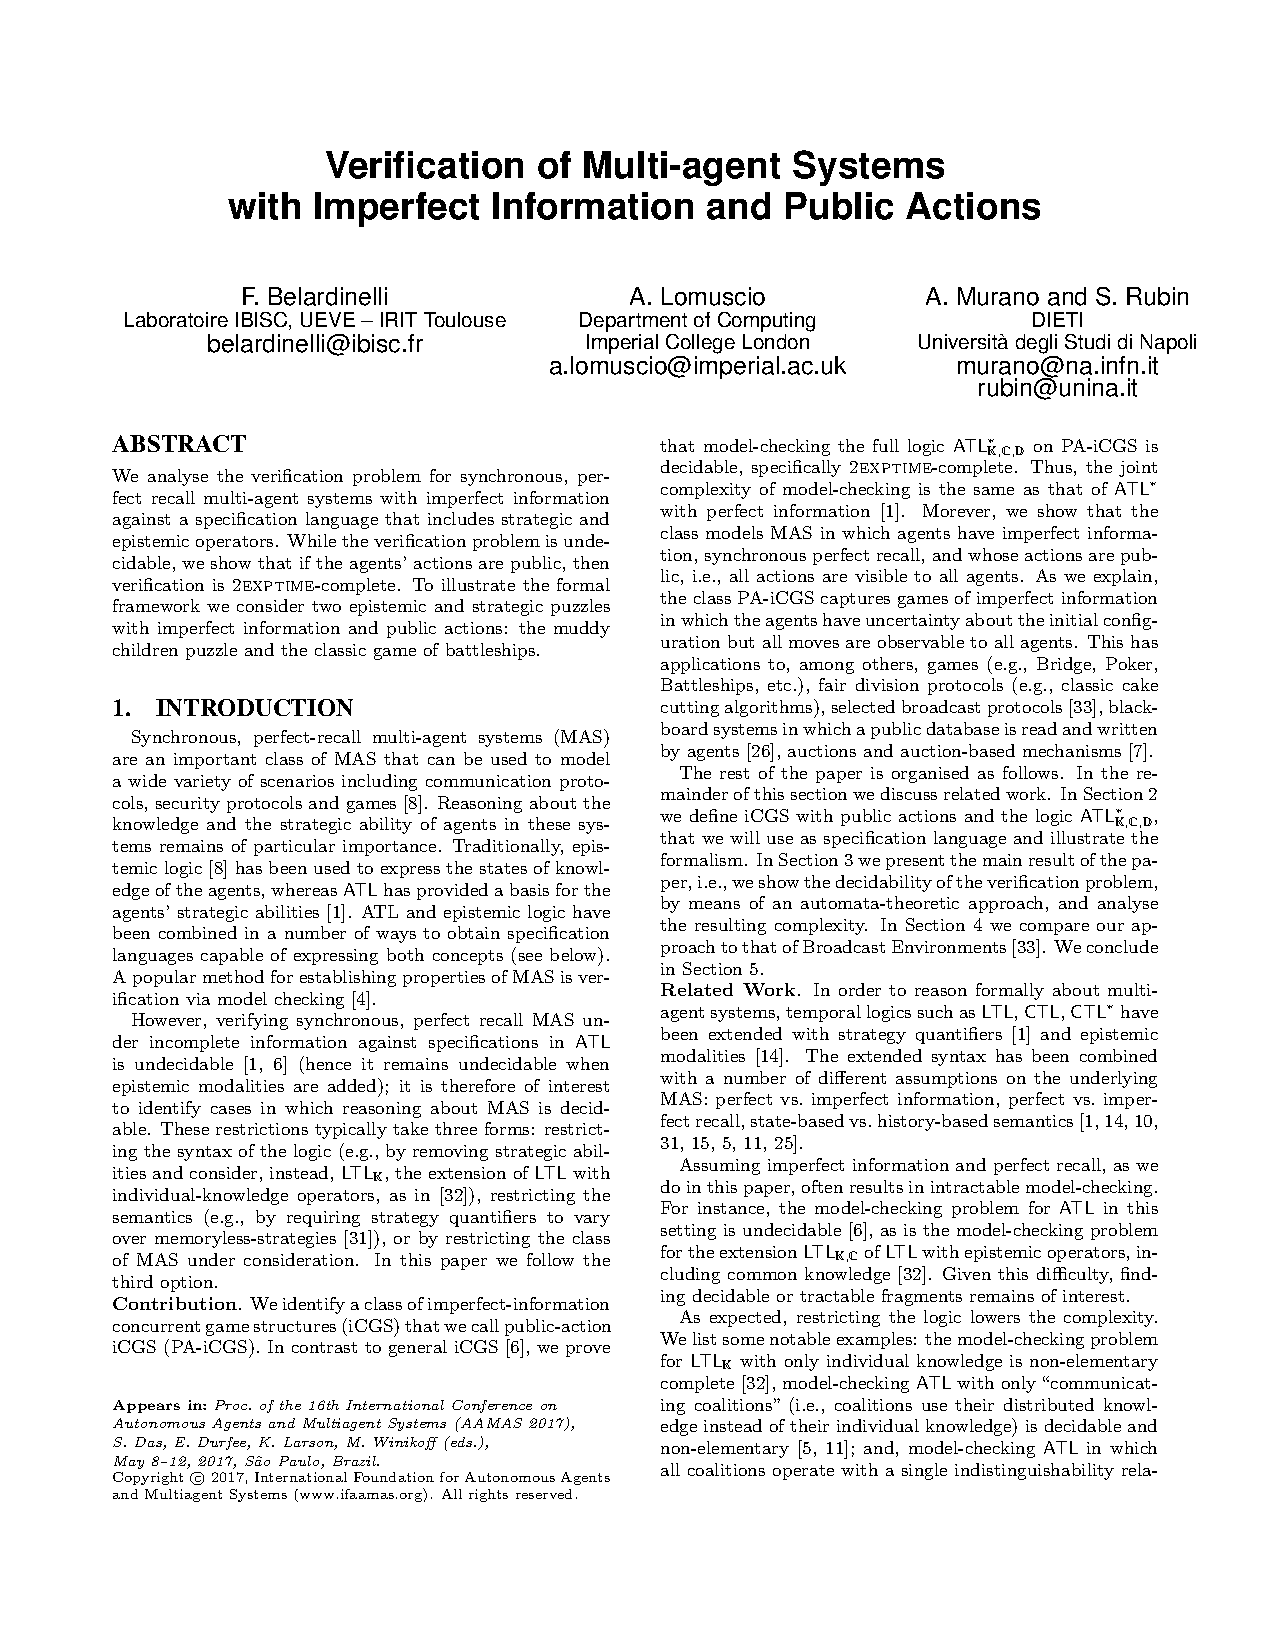
\includepdf[pages={-}]{no35.pdf}
\center \subsection{Publication} 
 \lb 
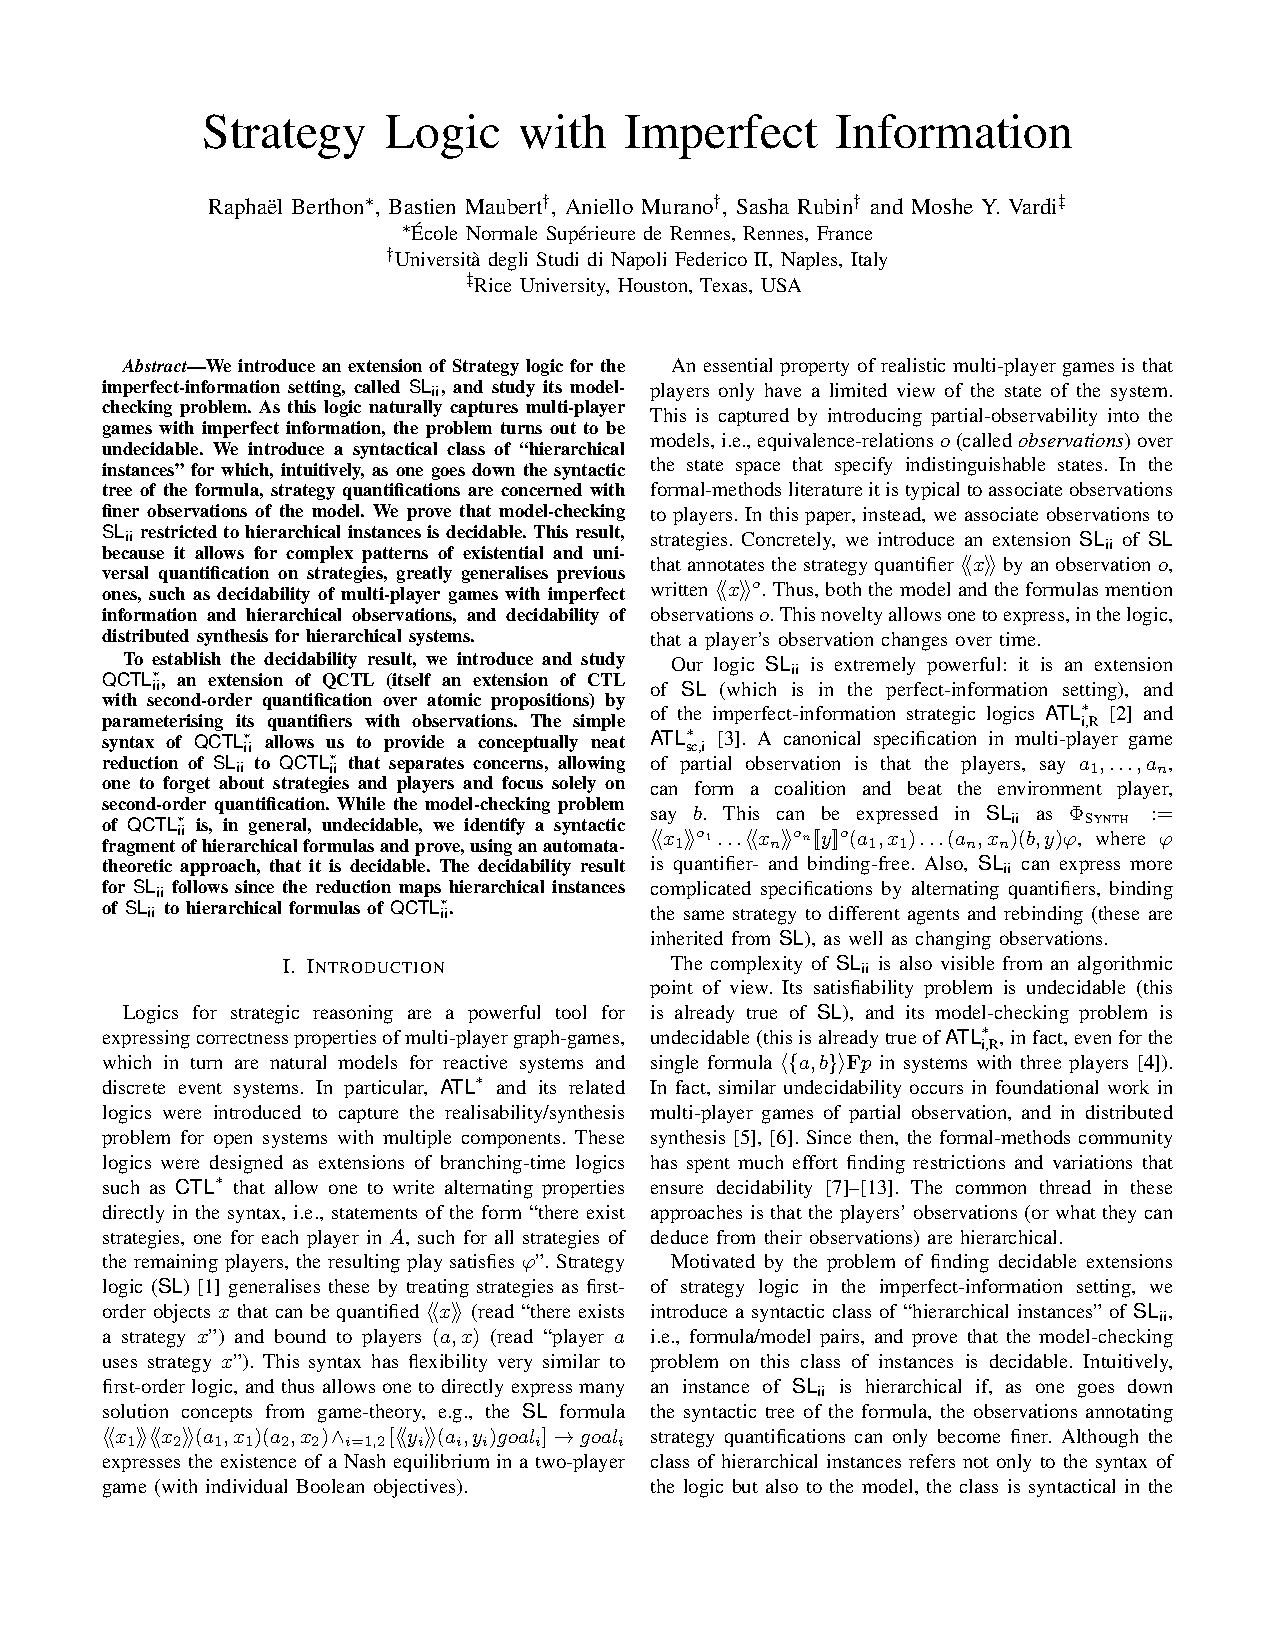
\includepdf[pages={-}]{no36.pdf}

 % {\center \section{Doctoral Thesis}}
%\addcontentsline{toc}{section}{Doctoral Thesis}

\end{document}
